\section{Statistical language model to WFST}
\label{sec:grmmod}

\subsection{$n-$gram Language Model Format}
\label{subsubsec:ngramformat}

The word level grammar G, often a stochastic $n-$gram, can be represented by WFST compactly~\cite{allauzen2003generalized}. The basic idea of constructing WFST from $n-$gram, can be described by the following rules (\href{http://openfst.cs.nyu.edu/twiki/bin/view/GRM/NGramModelFormat}{OpenGrm project NGram Model Format} by Michael Riley \textit{et al}.). \vspace{5mm}

An n-gram is a sequence of $k$ symbols: $w_1\cdots{}w_k$. Let $\mathbb{N}$ be the set of n-grams in the model.

\begin{itemize}
\item
  There is a \textit{unigram} state in every model, representing the empty string.
\item
  Every proper prefix of every n-gram in $\mathbb{N}$ has an associated state in the model.
\item
  The state associated with an n-gram $w_1\cdots{}w_k$ has a backoff transition (labeled with $\langle epsilon\rangle$) to the state associated with its suffix $w_2\cdots{}w_k$.
\item
  An n-gram $w_1\cdots{}w_k$ is represented as a transition, labeled with $w_k$, from the state associated with its prefix $w_1\cdots{}w_{k-1}$ to a destination state defined as follows:
  \begin{itemize}
  \item
    If $w_1\cdots{}w_k$ is a proper prefix of an $n-$gram in the model, then the destination of the transition is the state associated with $w_1\cdots{}w_k$.
  \item
    Otherwise, the destination of the transition is the state associated with the suffix $w_2\cdots{}w_k$.
  \end{itemize}
\item
  Start and end of the sequence are not represented via transitions in the automaton or symbols in the symbol table. Rather
  \begin{itemize}
  \item
    The start state of the automaton encodes the ``start of sequence'' $n-$gram prefix (commonly denoted $\langle s\rangle$).
  \item
    The end of the sequence (often denoted $\langle /s\rangle$) is included in the model through state final weights, i.e., for a state associated with an $n-$gram prefix $w_1\cdots{}w_k$, the final weight of that state represents the weight of the $n-$gram $w_1\cdots{}w_k \langle /s\rangle$.
  \end{itemize}
\end{itemize}

\newpage
There is a small but complete bigram language model in ARPA format. Notice that the probabilities are base 10 logarithms.

\begin{Verbatim}[frame=none, framesep=5mm]
\data\
ngram 1=4
ngram 2=6

\1-grams:
-99 <s> -0.39794
-0.69897 </s>
-0.39794 foo -0.60206
-0.39794 bar -0.60206

\2-grams:
-0.251812 <s> foo
-0.4436975 <s> bar
-0.6478175 foo foo
-0.139662 foo bar
-0.3716111 bar </s>
-0.3233064 bar foo

\end\
\end{Verbatim}

\begin{figure}[H]
  \centering
  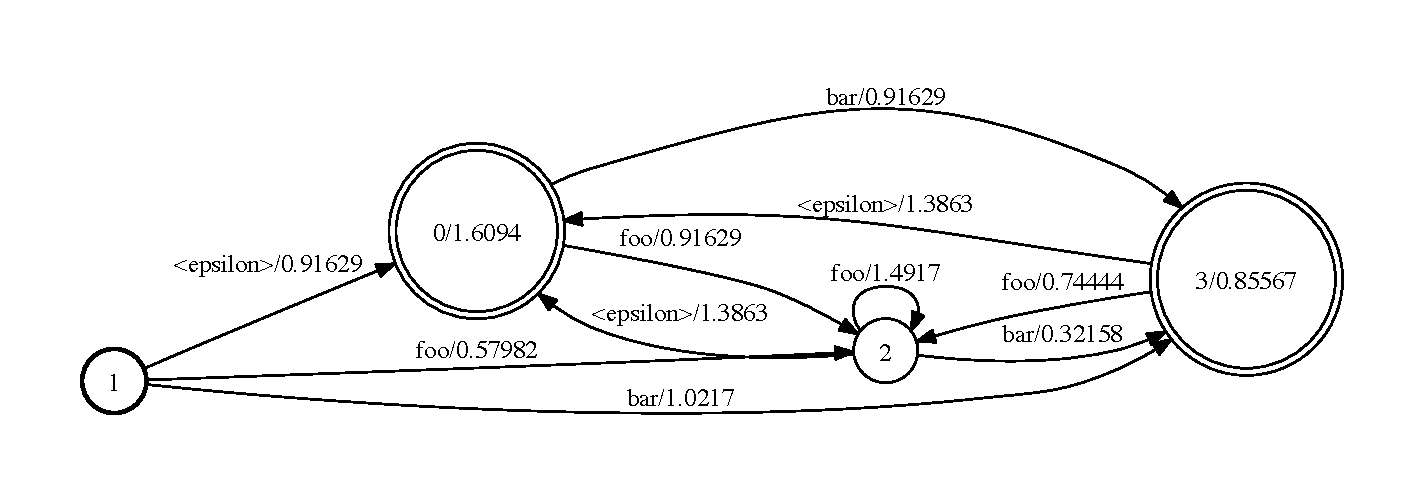
\includegraphics[width=\textwidth]{./figures/opengrm_2g.pdf}
  \caption{A bigram language model constructed by OpenGrm (ngrammake)}
\end{figure}

The model format used by Juicer and Transducersaurus is almost the same as OpenGrm NGram Format, except for

\begin{itemize}
\item
  There is a additional ``start'' state which only has one transition (labeled with $\langle s\rangle$) to the state associated with the ``start of sequence'' $n-$gram prefix (commonly denoted $\langle s\rangle$)
\item
  There is a additional ``end'' state (commonly denoted $\langle /s\rangle$). The end of the sequence (denoted $\langle /s\rangle$) is included in the model through a transition (labeled with $\langle /s\rangle$) to the ``end'' state. The weight of the transition represents the weight of the $n-$gram $w_1\cdots{}w_k \langle /s\rangle$. Thus, all successful paths are ended at this unique ``end'' state.
\end{itemize}

Figure~\ref{gramgen} depicts the G WFST constrcuted by gramgen.

\begin{figure}[H]
  \centering
  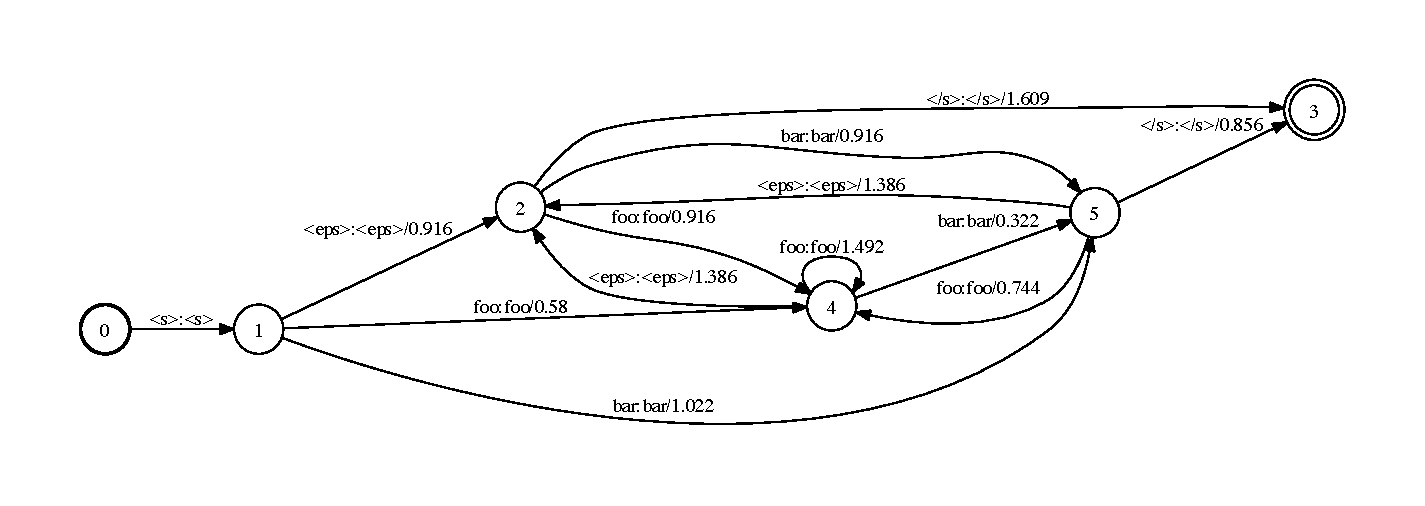
\includegraphics[width=\textwidth]{./figures/juicer_2g.pdf}
  \caption{A bigram language model constructed by Juicer (gramgen)}
  \label{gramgen}
\end{figure}

\subsection{Auxiliary Labels on Backoff $\epsilon-$Transitions}
\label{subsubsec:grmaux}
In the presence of backoff $\epsilon-$transitions, G may have several paths for a given word sequence. In this case, we can disambiguate the model by replacing the input $\epsilon-$label on backoff transitions with the auxiliary label (usually denoted by $\phi-$label). Respectively, We need to apply auxiliary symbols to L properly. By introducing auxiliary labels to G and L, we can ensure the composite WFST of L$^{*}$ (Kleene closure) and G is deterministic.

If we compose L$^{*}$ and G with matching filter without auxiliary symbols, we may get a non-deterministic and larger result as depicted in Figure~\ref{non-deterministic-LG}. An easier solution is using sequencing filter instead. Figure~\ref{deterministic-LG} shows the deterministic resulting WFST using sequencing filter, which can be optimized further.

Figure~\ref{lg_aux} shows that the same resulting WFST of composing L$^{*}$ and G by applying auxiliary symbols.

To reduce the size and facilitate the optimization of the composite WFST, it is encouraged to implement auxiliary symbols on L and G.

\begin{figure}[H]
  \centering
  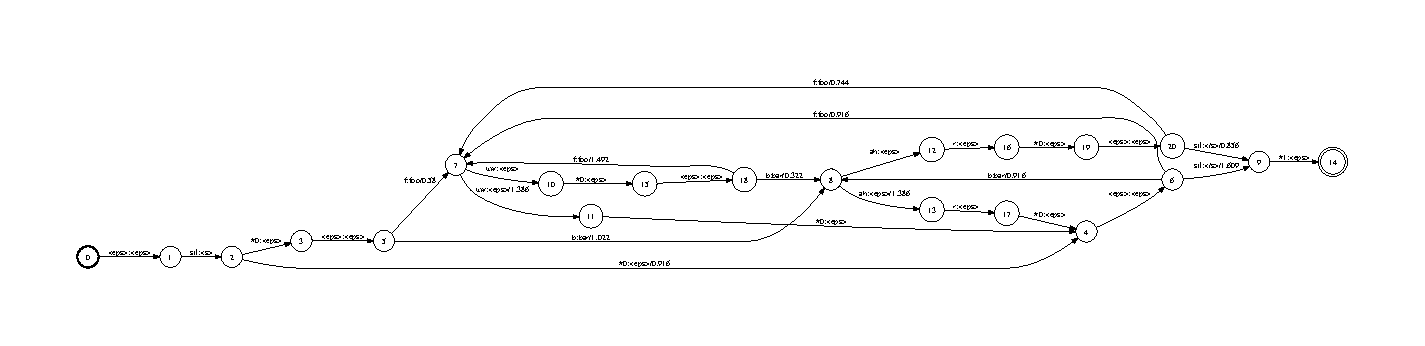
\includegraphics[width=\textwidth]{./figures/match_without_phi.pdf}
  \caption{Compose L$^{*}$ and G using matching filter, without auxiliary labels}
  \label{non-deterministic-LG}
\end{figure}

\begin{figure}[H]
  \centering
  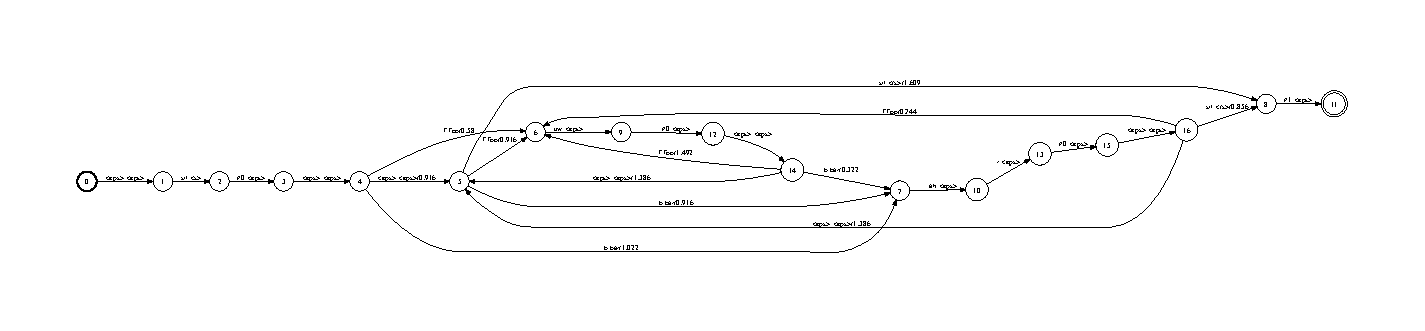
\includegraphics[width=\textwidth]{./figures/seq_without_phi.pdf}
  \caption{Compose L$^{*}$ and G using sequencing filter, without auxiliary labels}
  \label{deterministic-LG}
\end{figure}

\begin{figure}[H]
  \centering
  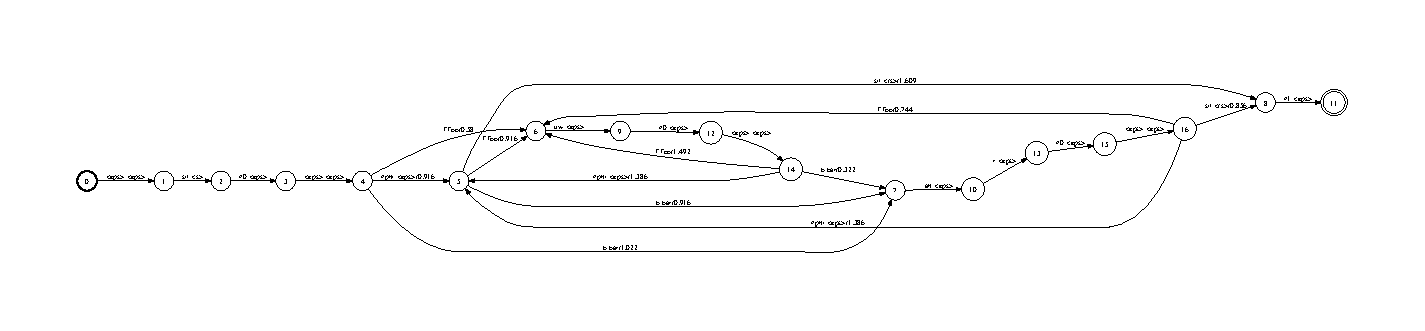
\includegraphics[width=\textwidth]{./figures/lg_with_phi.pdf}
  \caption{Compose L$^{*}$ and G, with auxiliary labels}
  \label{lg_aux}
\end{figure}


\subsection{$n-$gram Language Model Normalisation}
\label{subsubsec:grmnorm}
In practice, $n-$gram language models are trained on very large corpus. An unmodified language model is usually too large for practical use, so there are several pruning techniques to produce a smaller language model. However, some probability (seen $n-$grams) may be ``disgarded'' after pruning. To keep the stochasticity, the backoff weights need to be re-estimated. 

For example, the equation for Katz's backoff model~\cite{katz1987estimation} is
$$
\hat{P}(w_{i}|w_{i-n+1}\cdots{}w_{i-1}) = \left\{
\begin{aligned}
d_{w_{i-n+1}\cdots{}w_{i}}\frac{C(w_{i-n+1}\cdots{}w_{i})}{C(w_{i-n+1}\cdots{}w_{i-1})} \mbox{ if } C(w_{i-n+1}\cdots{}w_{i}) > k,\\
\alpha_{w_{i-n+1}\cdots{}w_{i-1}}\hat{P}(w_{i}|w_{i-n+2}\cdots{}w_{i-1}) \mbox{ otherwise.}\\
\end{aligned}
\right.
$$
where,

$C(x)$ is the number of times $x$ appears in training.

$w_{i}$ is the $i$th word in the given context.

$d$ is typically the amount of discounting found by Good-Turing estimation.

Thus the backoff weight $\alpha$ is computed as
$$
\alpha_{w_{i-n+1}\cdots{}w_{i-1}} = \frac{1-\sum\limits_{\{w_{i}:C(w_{i-n+1}\cdots{}w_{i})>k\}}d_{w_{i-n+1}\cdots{}w_{i}}\frac{C(w_{i-n+1}\cdots{}w_{i})}{C(w_{i-n+1}\cdots{}w_{i-1})}}{\sum\limits_{\{w_{i}:C(w_{i-n+1}\cdots{}w_{i})\leq{k}\}}\hat{P}(w_{i}|w_{i-n+2}\cdots{}w_{i-1})}
$$